\subsubsection{Giao diện người dùng - Danh sách/Chi tiết công ty}

Khi truy cập vào trang danh sách công ty, Front-end sẽ tự động fetch dữ liệu từ Backend thông qua một API tương tự như ở trang chủ: thực hiện phân trang để lấy lần lượt các công ty trong cơ sở dữ liệu dựa trên tham số \texttt{current} và \texttt{pageSize}.

\begin{figure}[H]
    \centering
    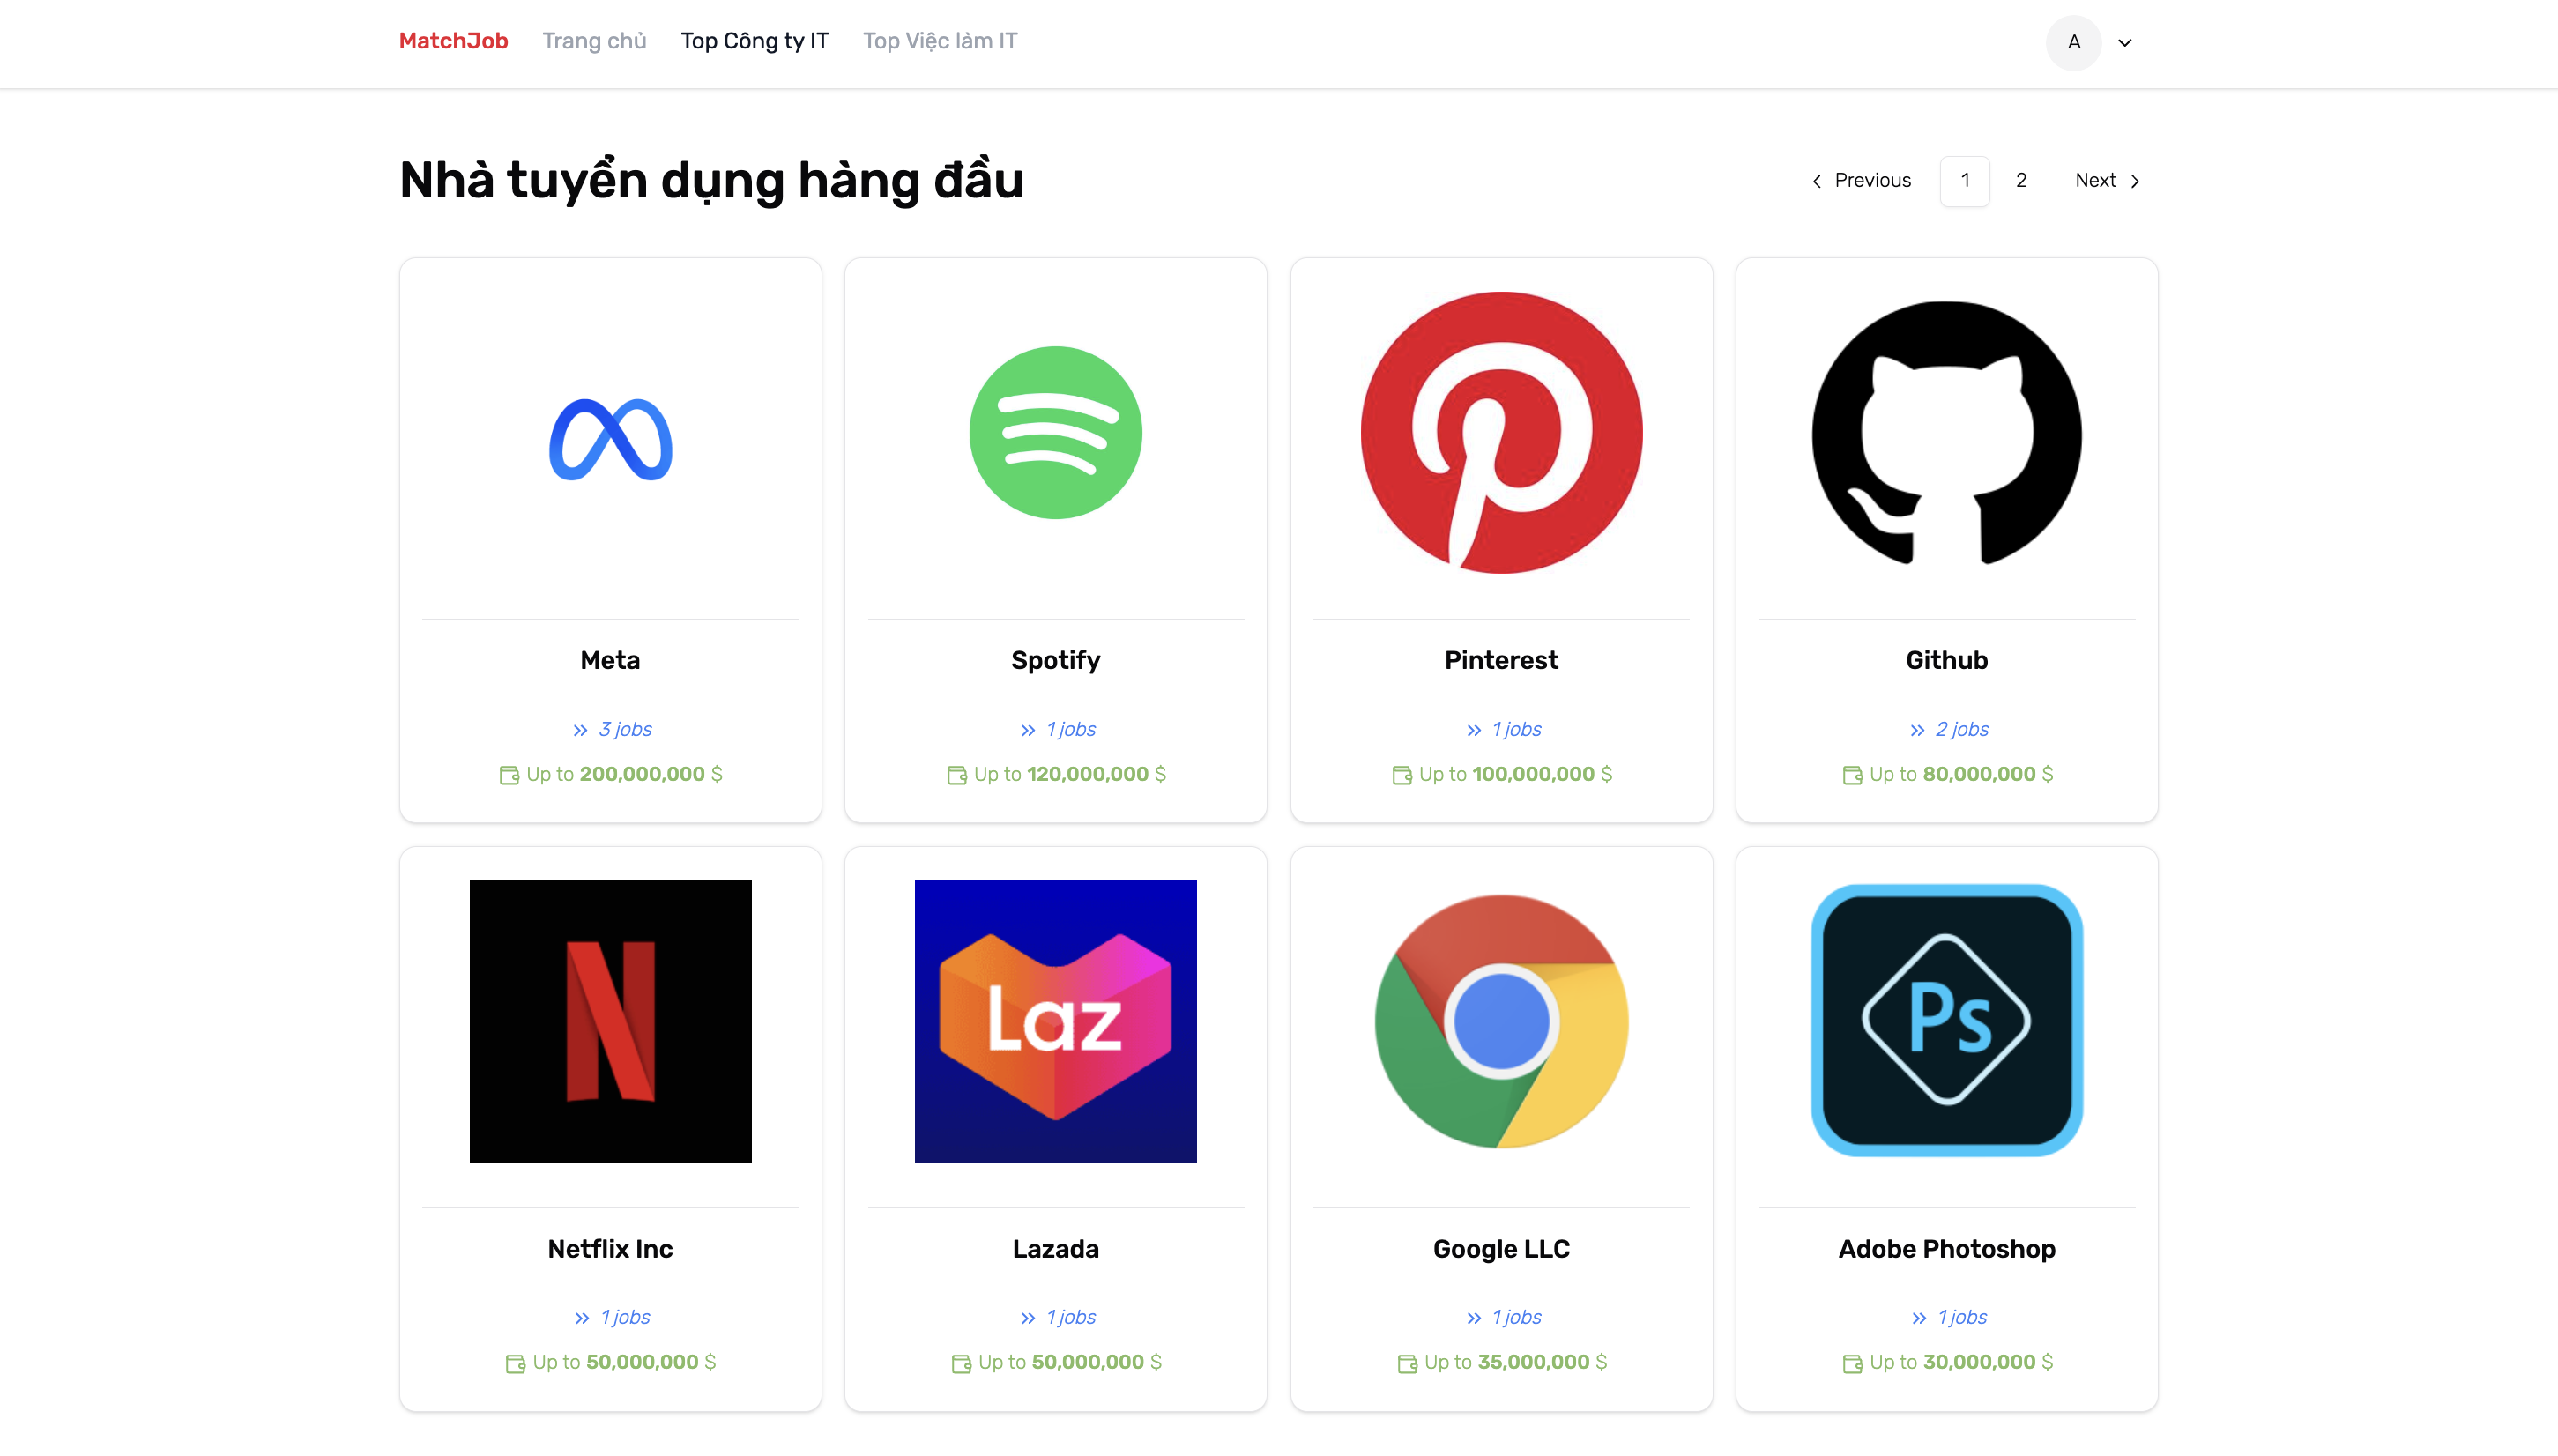
\includegraphics[width=\linewidth]{DBMS-Application/Images/list-company.png}
    \caption{Danh sách công ty}
    \label{fig:enter-label}
\end{figure}

Khi người dùng chọn 1 công ty trong danh sách, Front-end sẽ gửi yêu cầu đến API để lấy thông tin chi tiết của công ty đó và hiển thị lên giao diện người dùng:

\begin{figure}[H]
    \centering
    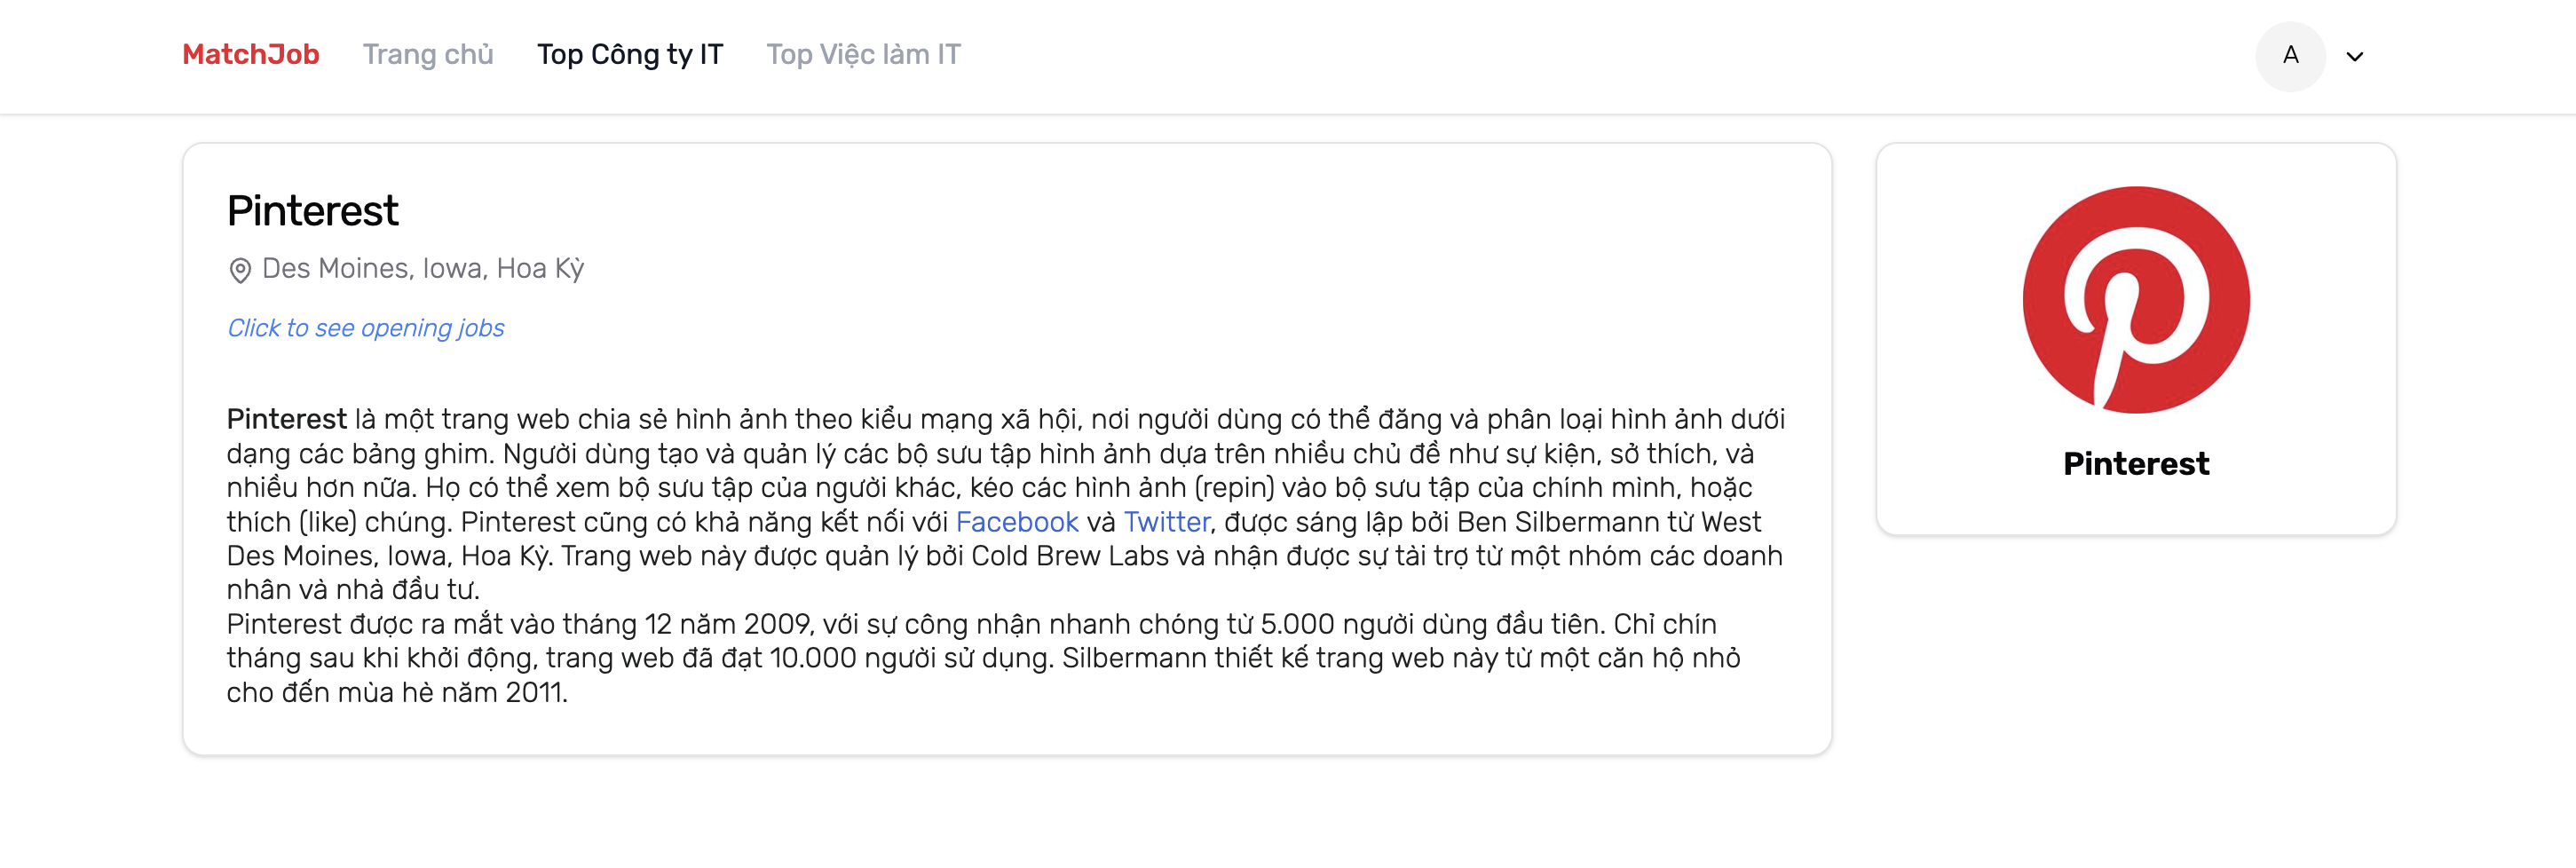
\includegraphics[width=\linewidth]{DBMS-Application/Images/company-detail.png}
    \caption{Thông tin chi tiết của công ty}
    \label{fig:enter-label}
\end{figure}

Truy vấn sử dụng: \textbf{Query with single condition} - Sử dụng điều kiện \texttt{\_id} để tìm công ty duy nhất

\begin{lstlisting}
return await this.db
  .collection('companies')
  .findOne({ _id: new ObjectId(id) }); // Chuyen id truyen vao thanh ObjectId, phu hop voi MongoDB
\end{lstlisting}

Ngoài ra, người dùng cũng có thể xem các công việc hiện đang được tuyển dụng của công ty này thông qua API lọc ra công việc của một công ty cụ thể (đã trình bày ở phần Trang chủ), hệ thống sẽ hiện lên 1 popup chứa các công việc của công ty hiện tại như sau:

\begin{figure}[H]
    \centering
    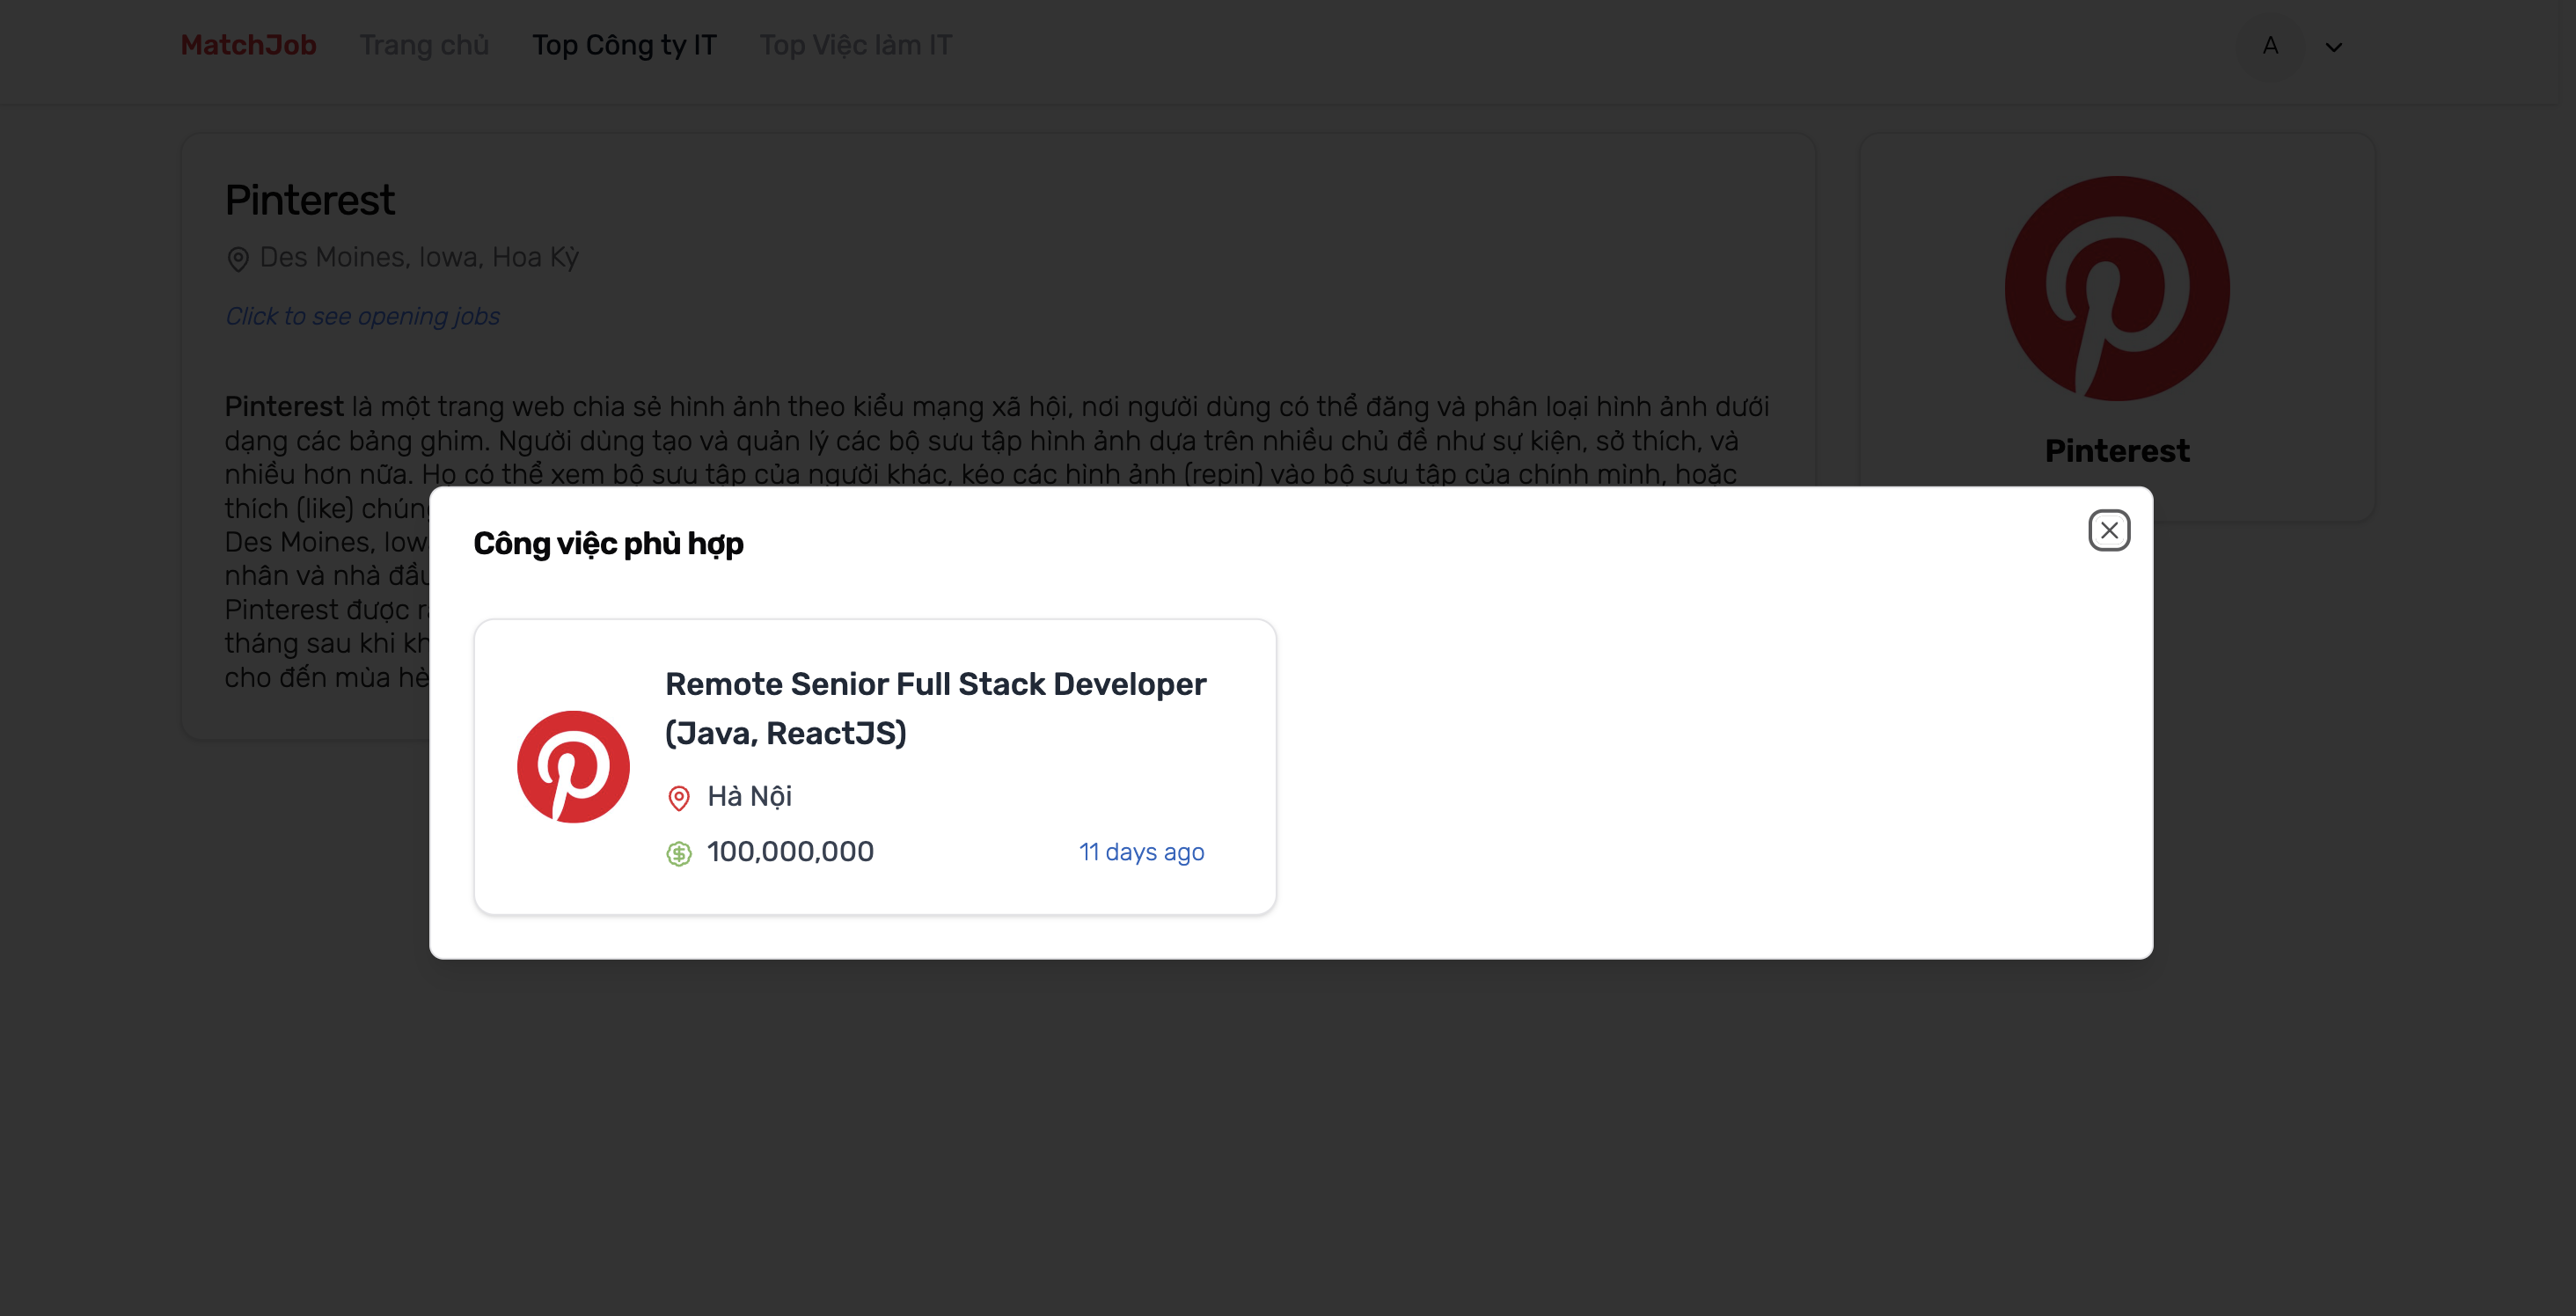
\includegraphics[width=\linewidth]{DBMS-Application/Images/modal-job-in-company-detail.png}
    \caption{Các công việc đang tuyển dụng của công ty cụ thể}
    \label{fig:enter-label}
\end{figure}


